% ============================================================
%  Demo for the "terminal" Beamer theme.
%  Compile with XeLaTeX or LuaLaTeX (twice, for the frame count).
%  On Overleaf: Menu > Settings > Compiler > XeLaTeX.
% ============================================================
\documentclass[aspectratio=169,10pt]{beamer}
\usetheme{terminal}            % options: nosectionpages, noprogressbar

\usepackage{amsmath,amssymb}
\usepackage{booktabs}
\usepackage{appendixnumberbeamer} % backup slides don't count in [nn/NN]
\usepackage{pgfplots}
\pgfplotsset{compat=1.18}
\usetikzlibrary{arrows.meta,positioning}

% ---------- theme settings ----------
\terminalfootprefix{demo}               % footline: "demo :: <short title>"
\terminalwindow{talk.tex}               % label in the title window bar
\terminalshell{%                        % fake shell session on the title page
  \$ make talk\\
  > compiling slides ............. ok\\
  > checking the coffee .......... ok}

\title[Terminal theme]{The Terminal Theme\\for Beamer}
\subtitle{Retro, monospaced, black and white}
\author{[Your Name]}
\institute{[Affiliation]}
\date{\today}

\begin{document}

\begin{frame}[plain,noframenumbering]
  \titlepage
\end{frame}

\begin{frame}{Agenda}
\begin{tbox}{> ls talk/}
\small
\begin{tabular}{@{}l@{\quad}l@{}}
01 & lists and text \\
02 & boxes \\
03 & tables, plots, diagrams \\
\end{tabular}
\end{tbox}
\end{frame}

% ============================================================
\section{LISTS AND TEXT}

\begin{frame}{Lists}
\begin{columns}[T]
\begin{column}{0.48\textwidth}
\begin{itemize}
\item items get a \textbf{>} prompt
  \begin{itemize}
  \item subitems get a dash
  \end{itemize}
\item \alert{alerted text} is bold, not coloured
\item math stays in Computer Modern: $\sum_{i=1}^{n} i = \tfrac{n(n+1)}{2}$
\end{itemize}
\end{column}
\begin{column}{0.48\textwidth}
\begin{enumerate}
\item enumerate uses brackets
\item like option flags
\item[\inv{!}] or anything you like
\end{enumerate}
\vskip8pt
\texttt{monospace everywhere}, \emph{even italics}.
\end{column}
\end{columns}
\src{Sources go bottom right with \texttt{\textbackslash src}}
\end{frame}

% ============================================================
\section{BOXES}

\begin{frame}{Boxes}
\begin{columns}[T]
\begin{column}{0.48\textwidth}
\begin{tbox}{tbox: a window with a title}
\small
\texttt{\textbackslash begin\{tbox\}\{title\}}\\
hard drop shadow, sharp corners
\end{tbox}
\vskip10pt
\begin{pbox}
\small
pbox: the same panel, without a title bar
\end{pbox}
\end{column}
\begin{column}{0.48\textwidth}
\begin{block}{block: Beamer's own}
\small
\texttt{block}, \texttt{alertblock} and \texttt{exampleblock} are restyled too
\end{block}
\vskip10pt
\begin{ibox}
ibox: an inverse-video banner
\end{ibox}
\vskip10pt
\centering\inv{3.6$\times$}\quad\inv{inline \textbackslash inv}
\end{column}
\end{columns}
\end{frame}

\begin{frame}{Overlays work as usual}
\begin{tbox}{> run -{}-step}
\small
\begin{itemize}
\item<1-> first this
\item<2-> then this
\item<3-> and finally this\,\terminalcursor
\end{itemize}
\end{tbox}
\end{frame}

% ============================================================
\section{TABLES AND PLOTS}

\begin{frame}{A table}
\centering\footnotesize
\begin{tabular}{@{}lrrr@{}}
\toprule
config & time (s) & memory (MB) & speed-up \\
\midrule
small  & 31.3  & 457  & \textbf{2.8} \\
medium & 52.6  & 946  & \textbf{2.8} \\
large  & 118.4 & 2505 & \textbf{3.6} \\
\bottomrule
\end{tabular}
\vskip14pt
\raggedright
\begin{itemize}\small
\item \texttt{booktabs} rules suit the black-and-white look
\end{itemize}
\end{frame}

\begin{frame}{A plot and a diagram}
\begin{columns}[c]
\begin{column}{0.55\textwidth}
\centering
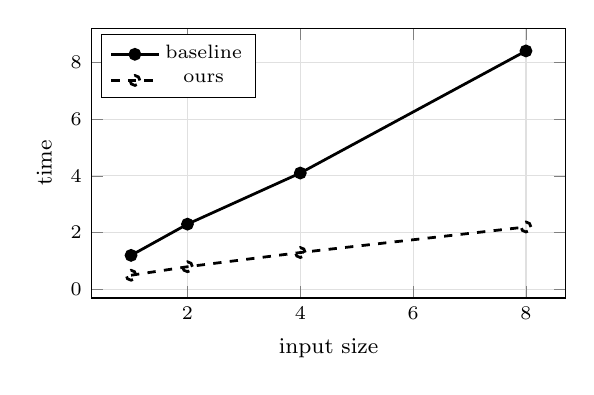
\begin{tikzpicture}
\begin{axis}[width=7.6cm,height=5cm,xlabel={input size},ylabel={time},
  tick label style={font=\scriptsize},label style={font=\footnotesize},
  legend style={font=\scriptsize,draw=black,at={(0.02,0.98)},anchor=north west},
  axis line style={line width=0.6pt},grid=major,grid style={black!12}]
\addplot[black,line width=1pt,mark=*,mark size=1.8pt] coordinates {(1,1.2)(2,2.3)(4,4.1)(8,8.4)};
\addlegendentry{baseline}
\addplot[black,line width=1pt,dashed,mark=o,mark size=1.8pt] coordinates {(1,0.5)(2,0.8)(4,1.3)(8,2.2)};
\addlegendentry{ours}
\end{axis}
\end{tikzpicture}
\end{column}
\begin{column}{0.42\textwidth}
\centering
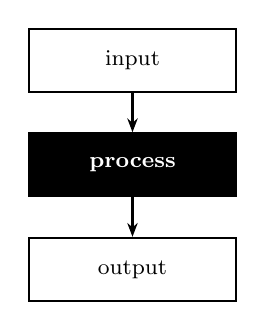
\begin{tikzpicture}[st/.style={draw=black,line width=0.8pt,minimum height=0.8cm,
    text width=2.4cm,align=center,font=\footnotesize,fill=white},
  arr/.style={-{Stealth[length=5pt]},line width=0.8pt}]
\node[st] (a) {input};
\node[st,fill=black,text=white,below=0.5cm of a] (b) {\textbf{process}};
\node[st,below=0.5cm of b] (c) {output};
\draw[arr] (a) -- (b); \draw[arr] (b) -- (c);
\end{tikzpicture}
\end{column}
\end{columns}
\end{frame}

% ============================================================
\terminalscreen{\$ talk -{}-questions}{QUESTIONS?}{[Your Name] \quad//\quad [email]}

\appendix
\section*{BACKUP}

\begin{frame}{Backup slide}
\begin{tbox}{note}
\small
after \texttt{\textbackslash appendix}, slides are not counted in the footline total
\end{tbox}
\end{frame}

\end{document}
